\subsection{Grenzwerte von Funktionen}
\subsubsection{Grenzwerte für \texorpdfstring{$x\rightarrow\pm\infty$}{x gegen unendlich}}
\begin{LA}
    {Einführungsaufgabe}{}
    \begin{enumerate}
        \item Nutzen Sie Geogebra, um den Graphen der Funktion $f(x)=\frac{3x^2+x-2}{2x^2-5x+8}$ zu skizzieren.
        \item Stellen Sie eine Vermutung auf: Was passiert mit den Werten der Funktion $f$, wenn der Input $x$ immer grösser wird?
        \item Untermauern Sie Ihre Vermutung, indem Sie die Gleichung von $f$ mit einer geschickten Termumformung verändern.
        \item Was passiert ganz links mit dem Graphen der Funktion $f$, also wenn $x$ gegen $-\infty$ strebt?
        \item Bestimmen Sie die beiden Grenzwerte $\lim\limits_{x\rightarrow\infty} g(x)$ und $\lim\limits_{x\rightarrow -\infty} g(x)$ der Funktion $$g(x)=\frac{2^x}{2^x+1}$$
    \end{enumerate}
\end{LA}
\clearpage
Die Werte der Funktion $f(x)=\frac{3x^2+x-2}{2x^2-5x+8}$ scheinen auf den ersten Blick für $x$ gegen $-\infty$ gegen die Zahl 1.5 zu streben. Diesen Eindruck kann man beispielsweise erhalten, wenn man sehr grosse Zahlen für $x$ einsetzt und feststellt, dass man Werte der Form $1.500000001$ erhält (siehe auch den Graphen unten). Allerdings kann man nicht ausschliessen, dass man für wirklich sehr grosse $x$ (z.B. $x=10^{(10^9)}$ die Grenze von $1.5$ unterschreiten wird; nicht zuletzt deshalb, weil es keinen Computer gibt, der zuverlässig mit solch grossen Zahlen rechnen kann – und es gibt noch viel, viel grössere Zahlen!

\begin{center}
    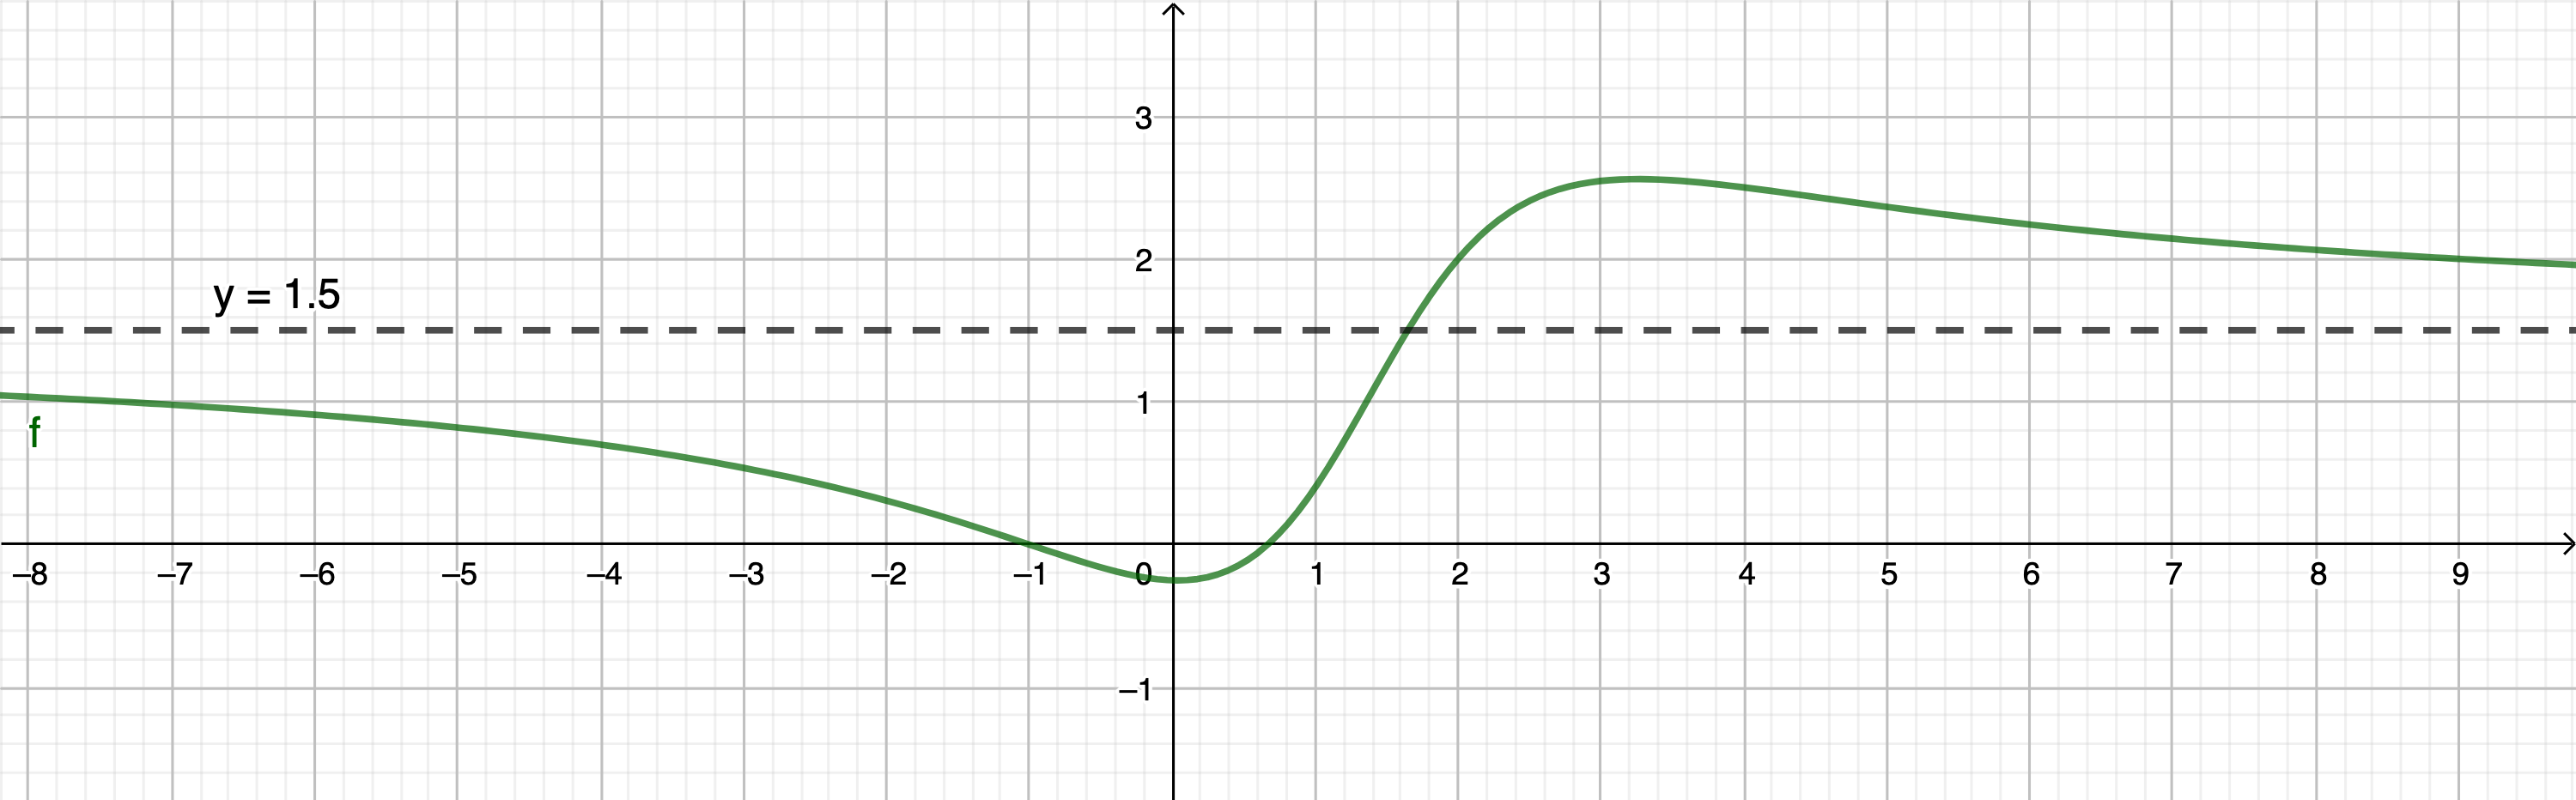
\includegraphics[scale=0.8]{media/introGrenzwertevonFu.png}
\end{center}
 
Ein Weg Gewissheit zu erlangen, ist eine Term-Analyse mit Hilfe einer Termumformung. Im konkreten Beispiel sieht das so aus:
$$f(x)=\frac{3x^2+x-2}{2x^2-5x+8}
=\frac{x^2\left(3+\frac{1}{x}-\frac{2}{x^2}\right)}{x^2 \left(2-\frac{5}{x}+\frac{8}{x^2}\right)}
=\frac{3+\frac{1}{x}-\frac{2}{x^2}}{2-\frac{5}{x}+\frac{8}{x^2}}$$ 

Für sehr grosse Werte von $x$ nähern sich die Terme $\frac{1}{x}, \frac{2}{x^2}, \frac{5}{x}$ und $\frac{8}{x^2}$  der Zahl $0$. Für $x\rightarrow\infty$ erhält man somit:
$$\lim_{x\rightarrow\infty} f(x) = \frac{3+0-0}{2-0+0} = \frac{3}{2}$$
Auf diese Art wird ersichtlich, dass sich die Funktion tatsächlich dem Grenzwert $1.5$ nähert.

Die Technik im Beispiel ist eine Anwendung der sogenannten Grenzwertsätzen:
 
\begin{satz}
    {Grenzwertsätze}{}
    Besitzen die Funktionen $f(x)$ und $g(x)$ Grenzwerte  für $x\rightarrow\infty$ so sind auch die Funktionen $f(x)\pm g(x),f(x)\cdot g(x)$ und, sofern $\lim\limits_{x\rightarrow\infty} g(x)\neq 0$, auch die Funktion $\frac{f(x)}{g(x)}$ konvergent.

Für die Grenzwerte gilt
$$\lim_{x\rightarrow\infty} (f(x) \pm g(x)) = \lim_{x\rightarrow\infty} f(x) \pm \lim_{x\rightarrow\infty}g(x)$$
$$\lim_{x\rightarrow\infty} (f(x) \cdot g(x)) = \lim_{x\rightarrow\infty} f(x) \cdot \lim_{x\rightarrow\infty}g(x)$$
$$\lim_{x\rightarrow\infty} \frac{f(x)}{g(x)} = \frac{\lim_{x\rightarrow\infty} f(x)}{\lim_{x\rightarrow\infty}g(x)}$$

Der Satz gilt auch für den Fall $x\rightarrow-\infty$
\end{satz}
Beweis: Siehe entsprechender Beweis im Kapitel „Folgen“...
\begin{ueb}
    {}{}
   \begin{enumerate}
    \item Bestimme, sofern vorhanden, den Grenzwert des Funktionsterms für $x \to \infty$.

    \begin{enumerate}
        \item $\lim\limits_{x \to \infty} \frac{x}{3x - 1}$
        \item $\lim\limits_{x \to \infty} \frac{1 - x^2}{x}$
        \item $\lim\limits_{x \to \infty} \frac{3x^7 - 4x^5}{2x^7 + 7x^6}$
        \item $\lim\limits_{x \to \infty} \frac{3 - x^3}{2x^3 + x^2}$
    \end{enumerate}
\item Welchen Wert hat $\lim\limits_{x \to \infty} f(x)$ und $\lim\limits_{x \to -\infty} f(x)$?

\begin{enumerate}
    \item $f(x) = \frac{2 + 3 \cdot 2^x}{2^x \cdot 4 - 1}$
    \item $f(x) = \frac{5^{-x} + 3}{8 - 2 \cdot 5^{-x}}$
\end{enumerate}

\item 
Berechne

\begin{enumerate}
    \item $\lim\limits_{x \to \infty} \frac{x^3 + \sin(x)}{x^3}$
    \item $\lim\limits_{x \to -\infty} \frac{x^2 - \sin(x)}{x^3}$
    \item $\lim\limits_{x \to \infty} \frac{\cos(x) - 3x}{1 - 2x}$
\end{enumerate}    
\item Bestimme die beiden Grenzwerte und vergleiche.

\begin{enumerate}
    \item $\lim\limits_{x \to \infty} \frac{2x^6 - 3x^5 + 7x^3 + 4x - 8}{5x^6 + 8x^5 - 9x^4 + 11x^2}$, \quad $\lim\limits_{x \to -\infty} \frac{2x^6 - 3x^5 + 7x^3 + 4x - 8}{5x^6 + 8x^5 - 9x^4 + 11x^2}$
    \item $\lim\limits_{x \to \infty} \frac{10x^8 - 4x^7 + 12}{x^9 + 3x^6 + 4}$, \quad $\lim\limits_{x \to -\infty} \frac{10x^8 - 4x^7 + 12}{x^9 + 3x^6 + 4}$
    \item  $\lim\limits_{x \to \infty} \frac{10x^8 - 4x^7 + 12}{x^7 + 3x^6 + 4}$, \quad $\lim\limits_{x \to -\infty} \frac{10x^8 - 4x^7 + 12}{x^7+ 3x^6 + 4}$
    \item   $\lim\limits_{x \to \infty} \frac{10x^8 - 4x^7 + 12}{ 3x^6 + 4}$, \quad $\lim\limits_{x \to -\infty} \frac{10x^8 - 4x^7 + 12}{3x^6 + 4}$
    \item $\lim\limits_{x \to \infty} \frac{\sqrt{x + 1}}{x - 1}$, \quad $\lim\limits_{x \to -\infty} \frac{\sqrt{x + 1}}{x - 1}$
    \item $\lim\limits_{x \to \infty} \frac{x^9 + x^4}{e^x}$, \quad $\lim\limits_{x \to -\infty} \frac{x^9 + x^4}{e^x}$
\end{enumerate}
\item Bestimme die Parameter $a, b$ und $c$ so, dass gilt:
    \[ \lim\limits_{x \to \infty} \frac{ax^b + 4x^5 + cx^3 - 1}{2x^3 - 11x^2 + 5} = 3. \]
\item  Gegeben ist der Funktionsterm $f(x) = \frac{4x^4 - 6x^3 + 7}{2x^m + 5x + 1}$. Bestimme den Exponenten $m \in \mathbb{N}_0$ so, dass die folgenden Grenzwerte resultieren, oder erkläre, weshalb es kein $m$ mit diesem Grenzwert gibt.
\begin{enumerate}
    \item $\lim\limits_{x \to \infty} f(x) = 2$
    \item $\lim\limits_{x \to \infty} f(x) = 0$
    \item $\lim\limits_{x \to -\infty} f(x) = -2$
    \item $\lim\limits_{x \to -\infty} f(x) = -\infty$
    \item $\lim\limits_{x \to -\infty} f(x) = \infty$
\end{enumerate}
   \end{enumerate}
\end{ueb}

\clearpage
\emph{Lösungen}
\begin{enumerate}
    \item 

\begin{enumerate}
    \item $\lim\limits_{x \to \infty} \frac{x}{3x - 1} = \frac{1}{3}$
    \item $\lim\limits_{x \to \infty} \frac{1 - x^2}{x} = -\infty$
    \item $\lim\limits_{x \to \infty} \frac{3x^7 - 4x^5}{2x^7 + 7x^6} = \frac{3}{2}$
    \item $\lim\limits_{x \to \infty} \frac{3 - x^3}{2x^3 + x^2} = -\frac{1}{2}$
\end{enumerate}

\item

\begin{enumerate}
    \item $f(x) = \frac{2 + 3 \cdot 2^x}{2^x \cdot 4 - 1}$, Grenzwert für $x\to \infty$: $\frac{3}{4}$, Grenzwert für $x\to-\infty$: $-2$
    \item $f(x) = \frac{5^{-x} + 3}{8 - 2 \cdot 5^{-x}}$, Grenzwert für $x\to \infty$: $\frac{3}{8}$, Grenzwert für $x\to-\infty$: $-\frac{1}{2}$
\end{enumerate}

\item

\begin{enumerate}
    \item $\lim\limits_{x \to \infty} \frac{x^3 + \sin(x)}{x^3} = 1$
    \item $\lim\limits_{x \to -\infty} \frac{x^2 - \sin(x)}{x^3} = 0$
    \item $\lim\limits_{x \to \infty} \frac{\cos(x) - 3x}{1 - 2x} = \frac{3}{2}$
\end{enumerate}

\item

\begin{enumerate}
    \item $\lim\limits_{x \to \infty} \frac{2x^6 - 3x^5 + 7x^3 + 4x - 8}{5x^6 + 8x^5 - 9x^4 + 11x^2} = \frac{2}{5}$, $\lim\limits_{x \to -\infty} \frac{2x^6 - 3x^5 + 7x^3 + 4x - 8}{5x^6 + 8x^5 - 9x^4 + 11x^2} = \frac{2}{5}$
    \item $\lim\limits_{x \to \infty} \frac{10x^8 - 4x^7 + 12}{x^9 + 3x^6 + 4} = 0$, $\lim\limits_{x \to -\infty} \frac{10x^8 - 4x^7 + 12}{x^9 + 3x^6 + 4} = 0$
    \item   $\lim\limits_{x \to \infty} \frac{10x^8 - 4x^7 + 12}{x^7 + 3x^6 + 4} = \infty$, \quad $\lim\limits_{x \to -\infty} \frac{10x^8 - 4x^7 + 12}{x^7+ 3x^6 + 4}=- \infty$
    \item   $\lim\limits_{x \to \infty} \frac{10x^8 - 4x^7 + 12}{ 3x^6 + 4}= \infty$, \quad $\lim\limits_{x \to -\infty} \frac{10x^8 - 4x^7 + 12}{3x^6 + 4}= \infty$
    \item $\lim\limits_{x \to \infty} \frac{\sqrt{x + 1}}{x - 1} = 0$, $\lim\limits_{x \to -\infty} \frac{\sqrt{x + 1}}{x - 1}$ gibt es nicht 
    \item $\lim\limits_{x \to \infty} \frac{x^9 + x^4}{e^x} = 0$, $\lim\limits_{x \to -\infty} \frac{x^9 + x^4}{e^x} = -\infty$
\end{enumerate}

\item $a = -4$, $b = 5$, $c = 6$.

\item    \begin{enumerate}
        \item $\lim\limits_{x \to \infty} f(x) = 2$, Lösung: $m = 4$
        \item $\lim\limits_{x \to \infty} f(x) = 0$, Lösung:  $m>4$ 
        \item $\lim\limits_{x \to -\infty} f(x) = -2$, Lösung: nicht möglich
        \item $\lim\limits_{x \to -\infty} f(x) = -\infty$, Lösung: $m\in \{0, 1, 3\}$
        \item $\lim\limits_{x \to -\infty} f(x) = \infty$, Lösung: $m =2$
    \end{enumerate}

\end{enumerate}














\clearpage
\subsubsection{Grenzwert einer Funktion an einer Stelle \texorpdfstring{$a\in \R$}{a}}
\begin{LA}
    {Einführungsaufgabe}{}
    Untersuchen Sie die Funktion $f(x)=\frac{x^3+10x^2-24x}{7x-14}$. 
        \begin{enumerate}
            \item Wieso ist die Funktion an der Stelle $x=2$ nicht definiert?
            \item Zeichnen Sie die Funktion mit \href{https://www.geogebra.org/calculator}{Geogebra}
            \item Definieren Sie in Geogebra einen `Laufpunkt' auf dem Graphen von $f$, indem Sie P=(a, f(a)) tippen. Geogebra erstellt automatisch einen Schieberegler, mit dem Sie die $x$-Koordinate von $P$ verändern können.
            \item  Beobachten Sie, was mit $P$ passiert, wenn $a$ sich der Zahl 2 nähert.
            \item  Was vermuten Sie ist der Wert des Grenzwertes $\lim\limits_{x\to 2} f(x)$?
            \item  Wie kann man diesen Grenzwert anhand der Funktionsgleichung berechnen?
            %\item  Wenn man etwas rauszoomt, sieht man, dass der Graph von $f$ eine bekannte Form hat. Können Sie das anhand der Funktionsgleichung erklären?
        \end{enumerate}



    % \begin{enumerate}
    %     \item Berechnen Sie einige Werte und füllen Sie die Wertetabelle: \newline
    %     \begin{center}
    %         \begin{tabular}{c||c|c|c|c}
    %             $x$ & $0$ & $1$ & $2$ & $3$ \\ \hline
    %         $f(x)$    &&&&   
    %         \end{tabular}
                  
    %     \end{center}
    %     \item Wie erklären Sie sich das spezielle Resultat?
    %     \item Füllen Sie auch die folgende Wertetabelle aus:
    %     \begin{center}
    %         \begin{tabular}{c||c|c|c|c}
    %             $x$ & $1.9$ & $1.99$ & $2.01$ & $2.1$ \\ \hline
    %         $f(x)$    &&&&   
    %         \end{tabular}
                  
    %     \end{center}
    %     \item 	Zeichnen Sie die Funktion mit Geogebra: 
    %     \begin{enumerate}
    %         \item Definieren Sie in Geogebra einen «Laufpunkt» auf dem Graphen von $f$, indem Sie P=(a, f(a)) tippen. Geogebra erstellt so automatisch einen Schieberegler, mit dem Sie die $x$-Koordinate von $P$ verändern können.
    %         \item  Beobachten Sie was mit $P$ passiert, wenn $a$ sich der Zahl 2 nähert.
    %         \item  Wenn man etwas rauszoomt, sieht man, dass der Graph von $f$ eine bekannte Form hat. Können Sie das anhand der Funktionsgleichung erklären?
    %     \end{enumerate}
        
    % \end{enumerate}
\end{LA}
\newpage
Mit der Einführungsaufgabe haben wir ein Beispiel dafür, wie man sich den Grenzwert einer Funktion für $x$ gegen eine Zahl vorstellen muss. Auch für diesen Grenzwertbegriff gibt es eine präzise, mathematische Definition, wir verzichten aber hier vorerst darauf und beschränken uns auf eine etwas ungenauere, dafür verständlichere Variante:

\begin{definition}
    {Grenzwert einer Funktion an einer Stelle $a\in \R$}{}
Eine Zahl $g$ heisst Grenzwert der Funktion $f$ für $x$ gegen $a$, falls alle Funktionswerte $f(x)$ beliebig wenig von $g$ abweichen, sobald $x$ entsprechend nahe bei $a$ liegt, aber verschieden von $a$ ist.
Notation:
$$\lim_{x\rightarrow a} f(x) = g$$
\end{definition}


Betrachten wir noch einmal das Einführungsbeispiel. Die Wertetabelle lässt vermuten, dass der Grenzwert $\lim\limits_{x\rightarrow 2} \frac{x^3+10x^2-24x}{7x-14} =4$ ist. Wie kann man aber Gewissheit erlangen? Schliesslich haben wir nur die Werte an den Stellen $1.99$ und $2.01$ betrachtet, aber es gibt Zahlen, die sich um viel weniger von $2$ unterscheiden – zum Beispiel $x=2+10^{-1000000000}$. 

Wieder hilft uns eine Termumformung:
$$\frac{x^3+10x^2-24x}{7x-14} = \frac{x(x^2+10x-24)}{7(x-2)} = \frac{x(x-2)(x+12)}{7(x-2)}\stackrel{x\neq 2}{=}\frac{x(x+12)}{7}$$

Die beiden Terme ganz links und ganz rechts liefern für alle Werte von $x$ das gleiche Resultat mit einer Ausnahme: Für $x=2$ ist der Term links nicht definiert, der rechts aber schon. Bildlich gesprochen stimmen die Graphen der beiden Funktionen $f(x)=\frac{x^3+10x^2-24x}{7x-14}$ und $g(x)=\frac{x(x+12)}{7}$ überall überein – nur das der Graph von $f$ an der Stelle $x=2$ ein Loch aufweist, während jener von $g$ durchgängig ist. 
Damit gilt
$$\lim_{x\rightarrow2} \frac{x^3+10x^2-24x}{7x-14} = \lim_{x\rightarrow2} \frac{x(x+12)}{7} =\frac{2\cdot (2+12)}{7} = 4$$

\begin{ueb}
    {}{}
    Bestimme den Grenzwert

    % \begin{enumerate}
    %     \item $\lim\limits_{x \to 2} \frac{4-x^2}{2 - x}$
    %     \item $\lim\limits_{x \to 1} \frac{10x^2 - 10}{1 - x}$
    %     \item $\lim\limits_{x \to 3} \frac{8x - 24}{x^2 - 9}$
    %     \item $\lim\limits_{x \to -2} \frac{x^2 + 3x + 2}{x^2 + 2x}$
    %     \item $\lim\limits_{x \to 1} \frac{x^2 + 1}{x - 2}$
    %     \item $\lim\limits_{x \to 0} \frac{x^2 - 1}{x - 2}$
    %     \item $\lim\limits_{x \to 2} \frac{x^2 - 4}{x - 2}$
    %     \item $\lim\limits_{x \to -4} \frac{x - 2}{x^2 - 4}$
    %     \item $\lim\limits_{x \to 3} \frac{x^2 - 4x + 3}{x^2 - 9}$
    %     \item $\lim\limits_{x \to 1} \frac{x^2 - 4x + 3}{x^2 - 9}$
    % \end{enumerate}

    \begin{enumerate}
        \item $\lim\limits_{x \to 1} \frac{x^2 + 4x - 5}{x^2 - 1}$
        \item $\lim\limits_{x \to 1} \frac{x^2 + 4x - 5}{x^2 - 2x + 1}$
        \item $\lim\limits_{x \to -9} \frac{x^2 + 7x - 18}{x^2 - 81}$
        \item $\lim\limits_{x \to -4} \frac{x + 6}{x^2 - 4}$
        \item $\lim\limits_{x \to -2} \frac{12x^2 + 24x}{x^2 + 10x + 16}$
        \item $\lim\limits_{x \to 2} \frac{3x^2 - 6x}{6 - 5x + x^2}$
        \item $\lim\limits_{x \to 4} \frac{2x^2 - 14x + 24}{12x - 7x^2 + x^3}$
    \end{enumerate}
\end{ueb}
\clearpage
\emph{Lösungen}
% \begin{enumerate}
%     \item $\-4$
%     \item $\lim\limits_{x \to 1} \frac{10(x - 1)(x + 1)}{1 - x} = -10(1 + 1) = -20$
%     \item $\lim\limits_{x \to 3} \frac{8(x - 3)}{x^2 - 9} = \frac{8(3-3)}{9-9} = \text{nicht definiert}$
%     \item $\lim\limits_{x \to -2} \frac{x^2 + 3x + 2}{x^2 + 2x} = \frac{4 - 6 + 2}{4 - 4} = \text{nicht definiert}$
%     \item $\lim\limits_{x \to 1} \frac{x^2 + 1}{x - 2} = \frac{1 + 1}{1 - 2} = -2$
%     \item $\lim\limits_{x \to 0} \frac{x^2 - 1}{x - 2} = \frac{0 - 1}{-2} = \frac{1}{2}$
%     \item $\lim\limits_{x \to 2} \frac{x^2 - 4}{x - 2} = \lim\limits_{x \to 2} (x+2) = 4$
%     \item $\lim\limits_{x \to -4} \frac{x - 2}{x^2 - 4} = \frac{-4 - 2}{16 - 4} = \frac{-6}{12} = -\frac{1}{2}$
%     \item $\lim\limits_{x \to 3} \frac{x^2 - 4x + 3}{x^2 - 9} = \frac{9 - 12 + 3}{9 - 9} = \text{nicht definiert}$
%     \item $\lim\limits_{x \to 1} \frac{x^2 - 4x + 3}{x^2 - 9} = \frac{1 - 4 + 3}{1 - 9} = \frac{0}{-8} = 0$
% \end{enumerate}

\begin{enumerate}
    \item $3$
    \item unbestimmt divergent $\pm\infty$
    \item $\frac{11}{18}$
    \item $\frac{1}{6}$
    \item $-4$
    \item $-6$
    \item $1/2$
\end{enumerate}
















\clearpage

\subsubsection{Linksseitige und rechtsseitige Grenzwerte, Stetigkeit}

\begin{LA}{Einführungsaufgabe}{}
    Wir untersuchen die Funktion:
    $$f(x) = x\cdot \sqrt{1+\frac{1}{x^2}}$$

    \begin{enumerate}
        \item An welcher Stelle ist die Funktion nicht definiert?
        \item Was passiert, wenn $x$ sich der Definitionslücke nähert?
        \item Zeichnen Sie den Graphen von $f$ mit Geogebra und fügen Sie ihn hier unten an (Wurzeln können mit dem Befehl \glqq sqrt\grqq{} oder mit \glqq hoch 0.5\grqq{} eingegeben werden). 
    \end{enumerate}
\end{LA}
\clearpage
Für die Funktion aus der Einführungsaufgabe gilt: Je nachdem ob $x$ von links oder rechts gegen $0$ strebt, strebt der Funktionswert gegen $-1$ oder $+1$. Man spricht in diesem Fall vom links- bzw. rechtsseitigen Grenzwert und schreibt:
$$\lim_{x\uparrow 0} f(x) = -1 \quad \mathrm{oder}  \lim_{x\rightarrow 0^-} f(x) = -1 $$
beziehungsweise
$$\lim_{x\downarrow 0} f(x) = 1 \quad \mathrm{oder}  \lim_{x\rightarrow 0^+} f(x) = 1 $$

Für Funktionen gibt es an einer bestimmten Stelle drei mögliche Grenzwerte: der linksseitige, der rechtsseitige und DER Grenzwert. Der folgende Satz erklärt den Zusammenhang zwischen den drei Arten:

\begin{satz}{Zusammenhang zwischen den Grenzwerten}{}
Wenn der links- und der rechtsseitige Grenzwert übereinstimmen, dann existiert auch DER Grenzwert und es gilt:
$$\lim_{x\uparrow a} f(x) = \lim_{x\downarrow a} f(x) = \lim_{x\rightarrow a} f(x) $$

Wenn links- und rechtsseitige Grenzwerte \emph{nicht} übereinstimmen, dann existiert DER Grenzwert nicht.
$$\lim_{x\uparrow a} f(x) \neq \lim_{x\downarrow a} f(x) \Rightarrow  \lim_{x\rightarrow a} f(x) \text{ existiert nicht}$$
\end{satz}

\begin{bsp}
    {}{}
    Die Aufrundungsfunktion $x\mapsto \left \lceil{x}\right \rceil $ rundet jede Zahl $x$ auf die kleinste ganze Zahl, die grösser oder gleich $x$ ist.

    $\lim_{x\uparrow 42} \lceil x\rceil = ? , \quad \lim_{x\downarrow 42} \lceil x\rceil = ? $, Graph?
    
    \vspace{9cm}
\end{bsp}
\clearpage
Die Aufrundungsfunktion ist ein Beispiel für eine Funktion, die an gewissen Stellen Sprünge aufweist. Die meisten Funktionen, die Sie bisher angetroffen haben, hatten keine solche Sprungstellen. Wenn eine Funktion keine Sprungstelle hat, nennt man sie stetig. Genauer:

\begin{definition}{}{}
    Eine Funktion mit Definitionsbereich $\mathbb{D}$  heisst \emph{stetig an der Stelle $a\in \mathbb{D}$}, wenn
    $$ \lim_{x\uparrow a} f(x) = \lim_{x\downarrow a} f(x) = f(a)$$
\end{definition}
\begin{bsp}{}{}
    \begin{enumerate}
        \item Die Quadratfunktion $f(x)=x^2$ ist stetig. Der Graph weist keinerlei Sprungstellen auf.
        \begin{center}
            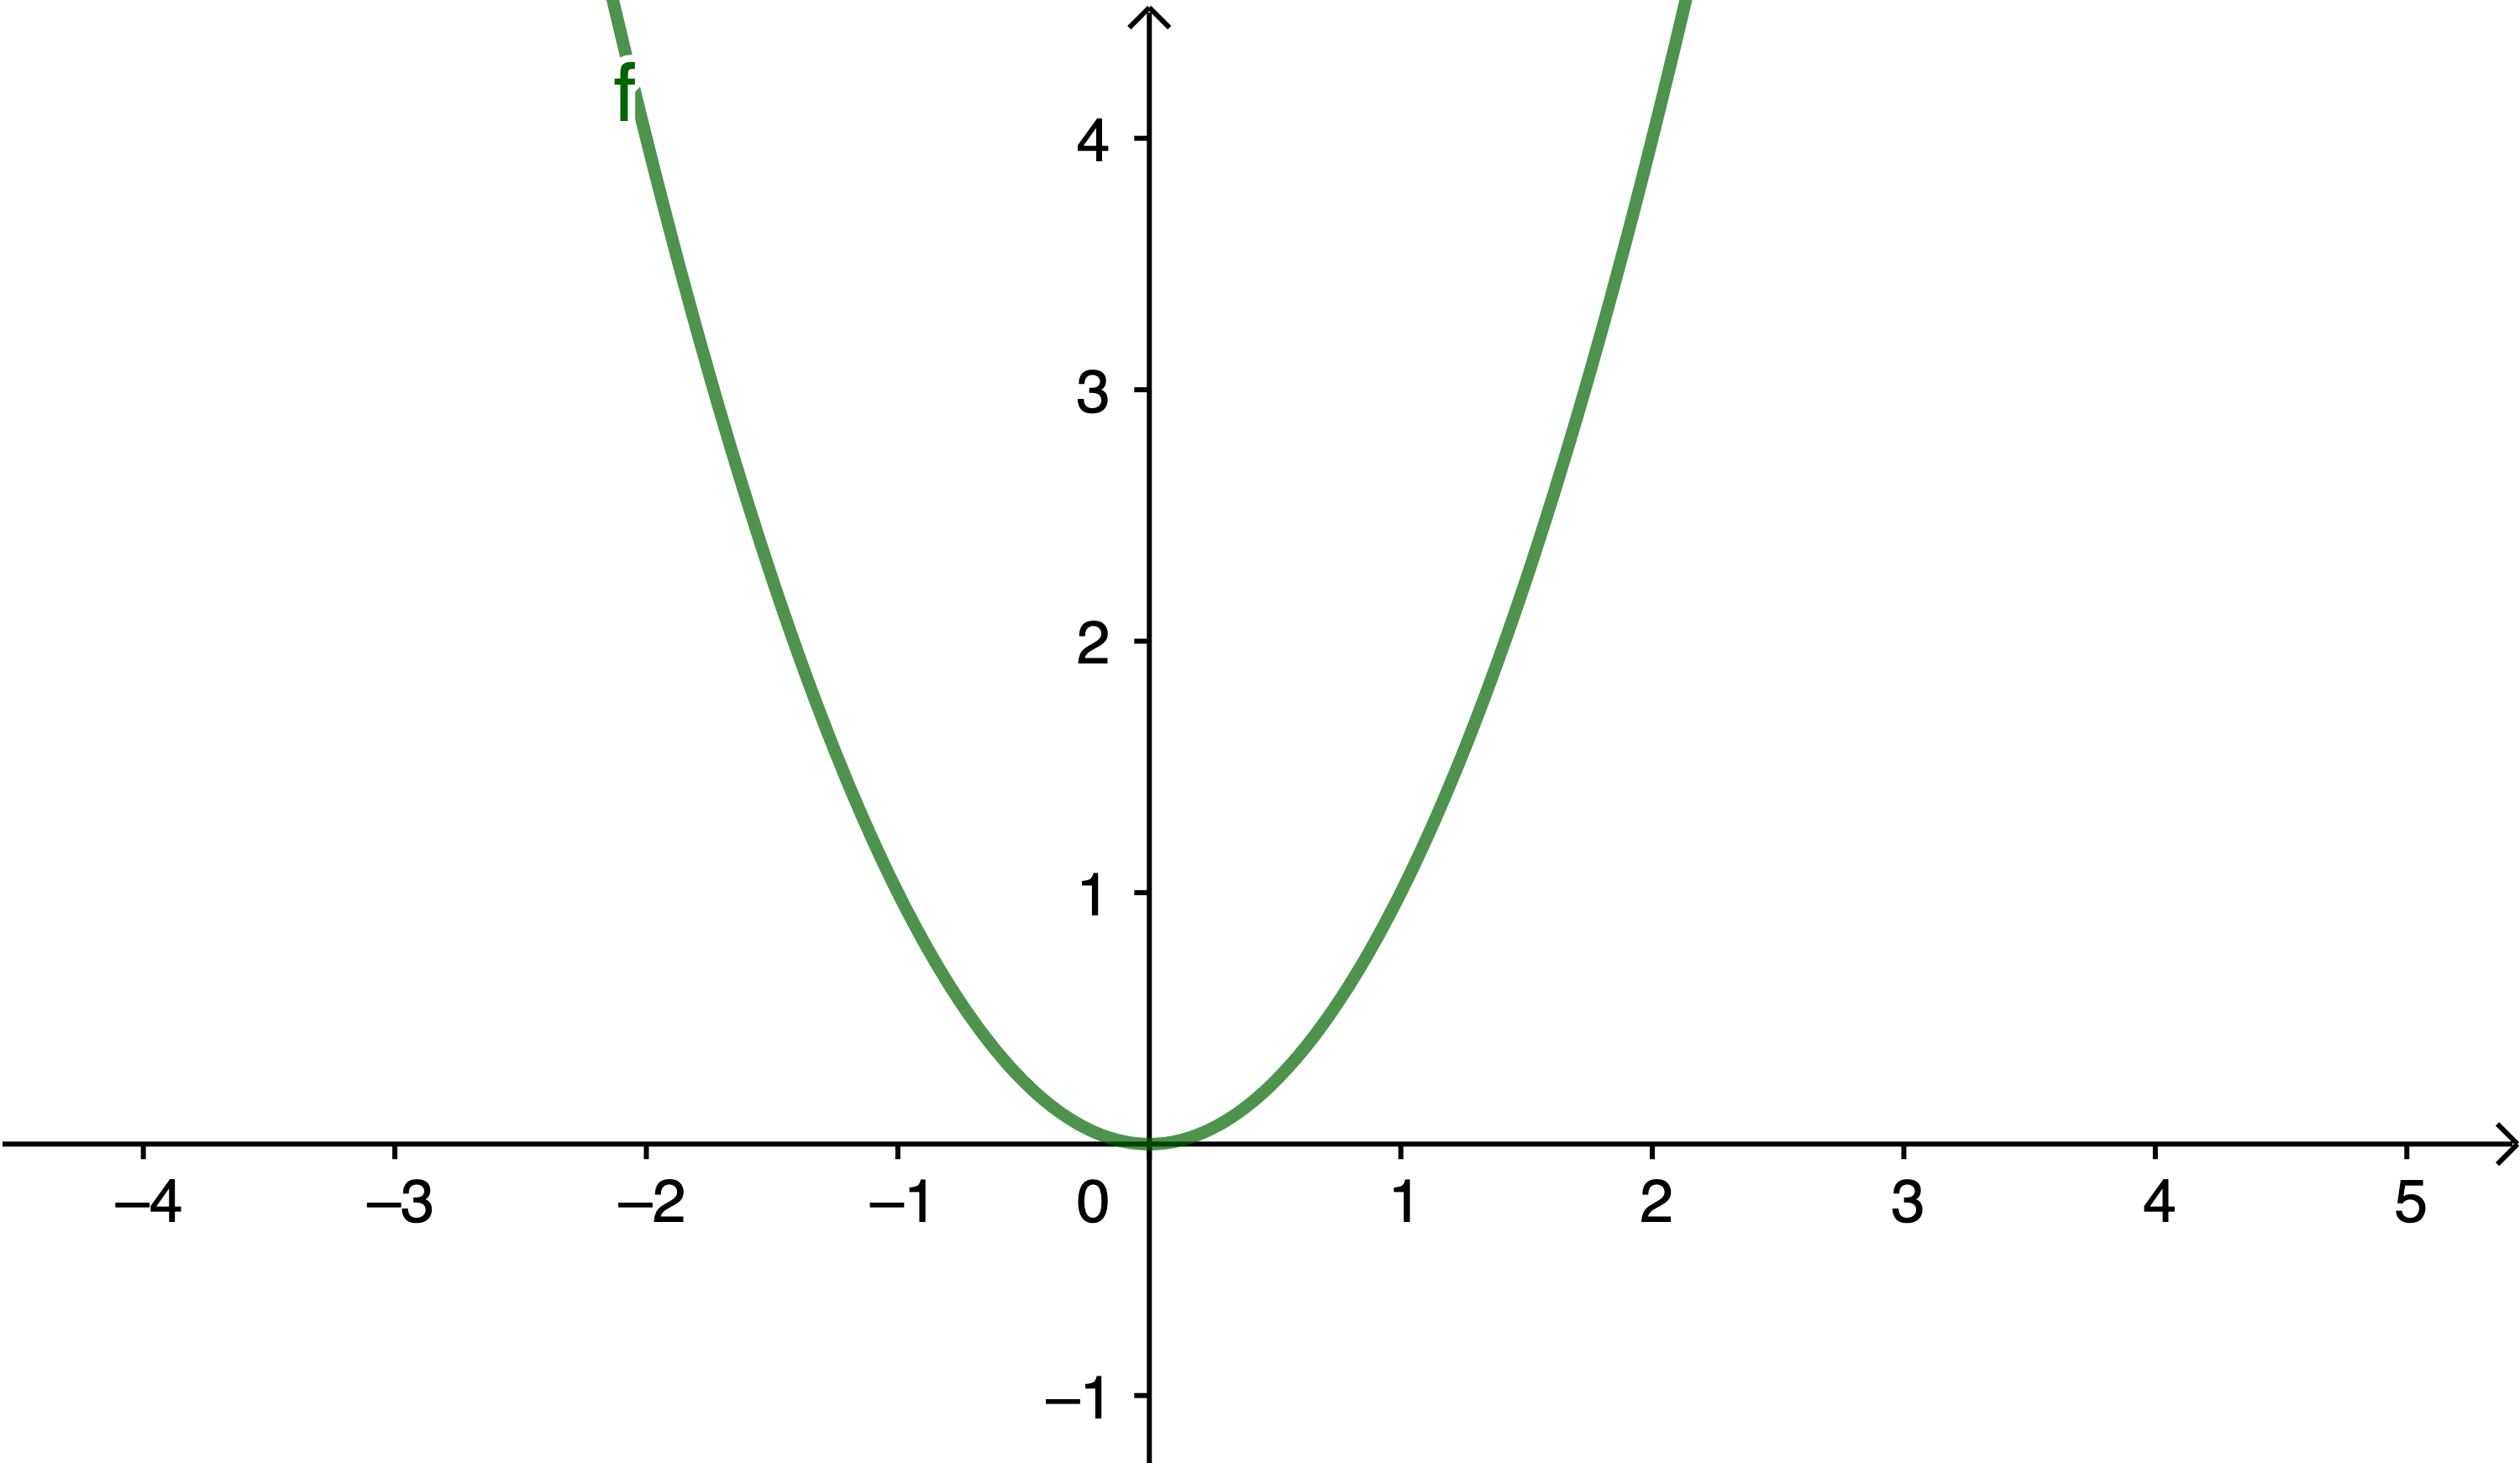
\includegraphics[scale=0.8]{media/quadratfunktion.png}
        \end{center}
    \item Die Vorzeichenfunktion 
    $$ \mathrm{sgn}(x)=\begin{cases}
        1, \quad \text{falls } x>0 \\
        0, \quad \text{falls } x=0 \\
        -1, \quad \text{falls } x<0
    \end{cases}$$
    ist nicht stetig, weil $$\lim_{x\uparrow 0} f(x) = -1 \neq \lim_{x\downarrow 0} f(x) = 1$$
    \begin{center}
        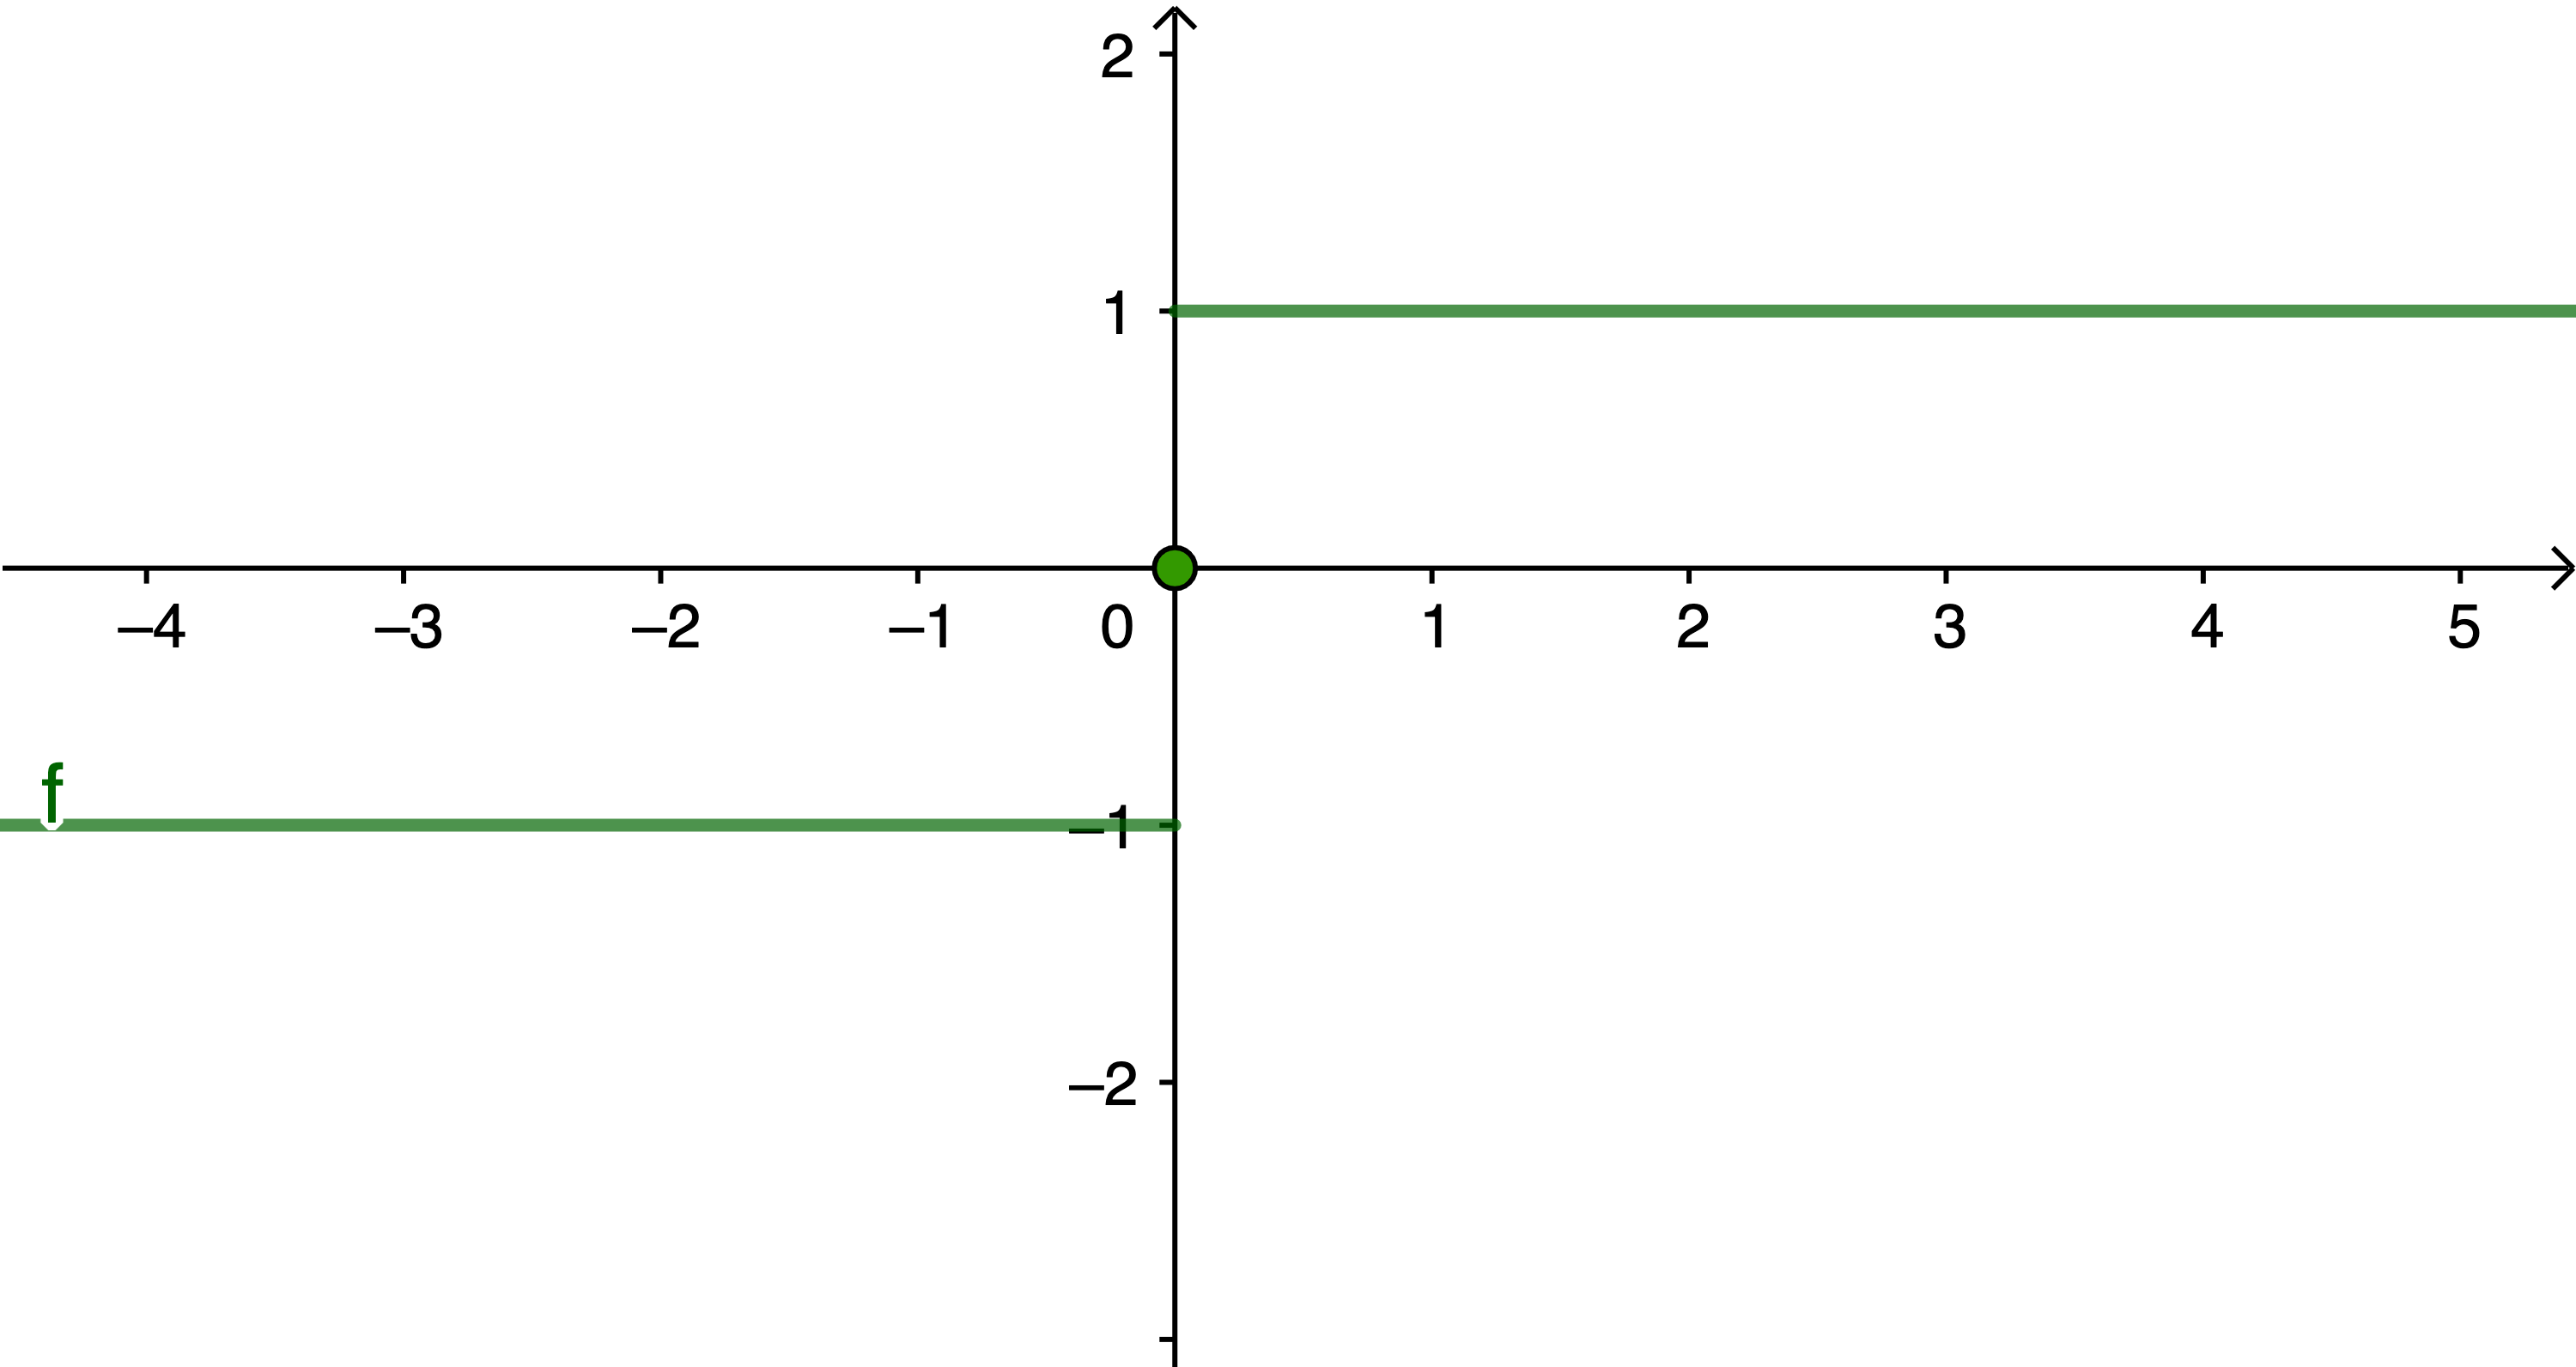
\includegraphics[scale=0.8]{media/sgn.png}
    \end{center}
    \pagebreak
    \item Die Betragsfunktion
    $$|x| = \begin{cases}
        x\quad \text{falls } x\le0 \\
        -x, \quad \text{falls } x<0 
    \end{cases}
    $$
    ist stetig. Der Graph hat zwar einen Ecke, aber keine \glqq Sprungstelle\grqq{}.
    \begin{center}
        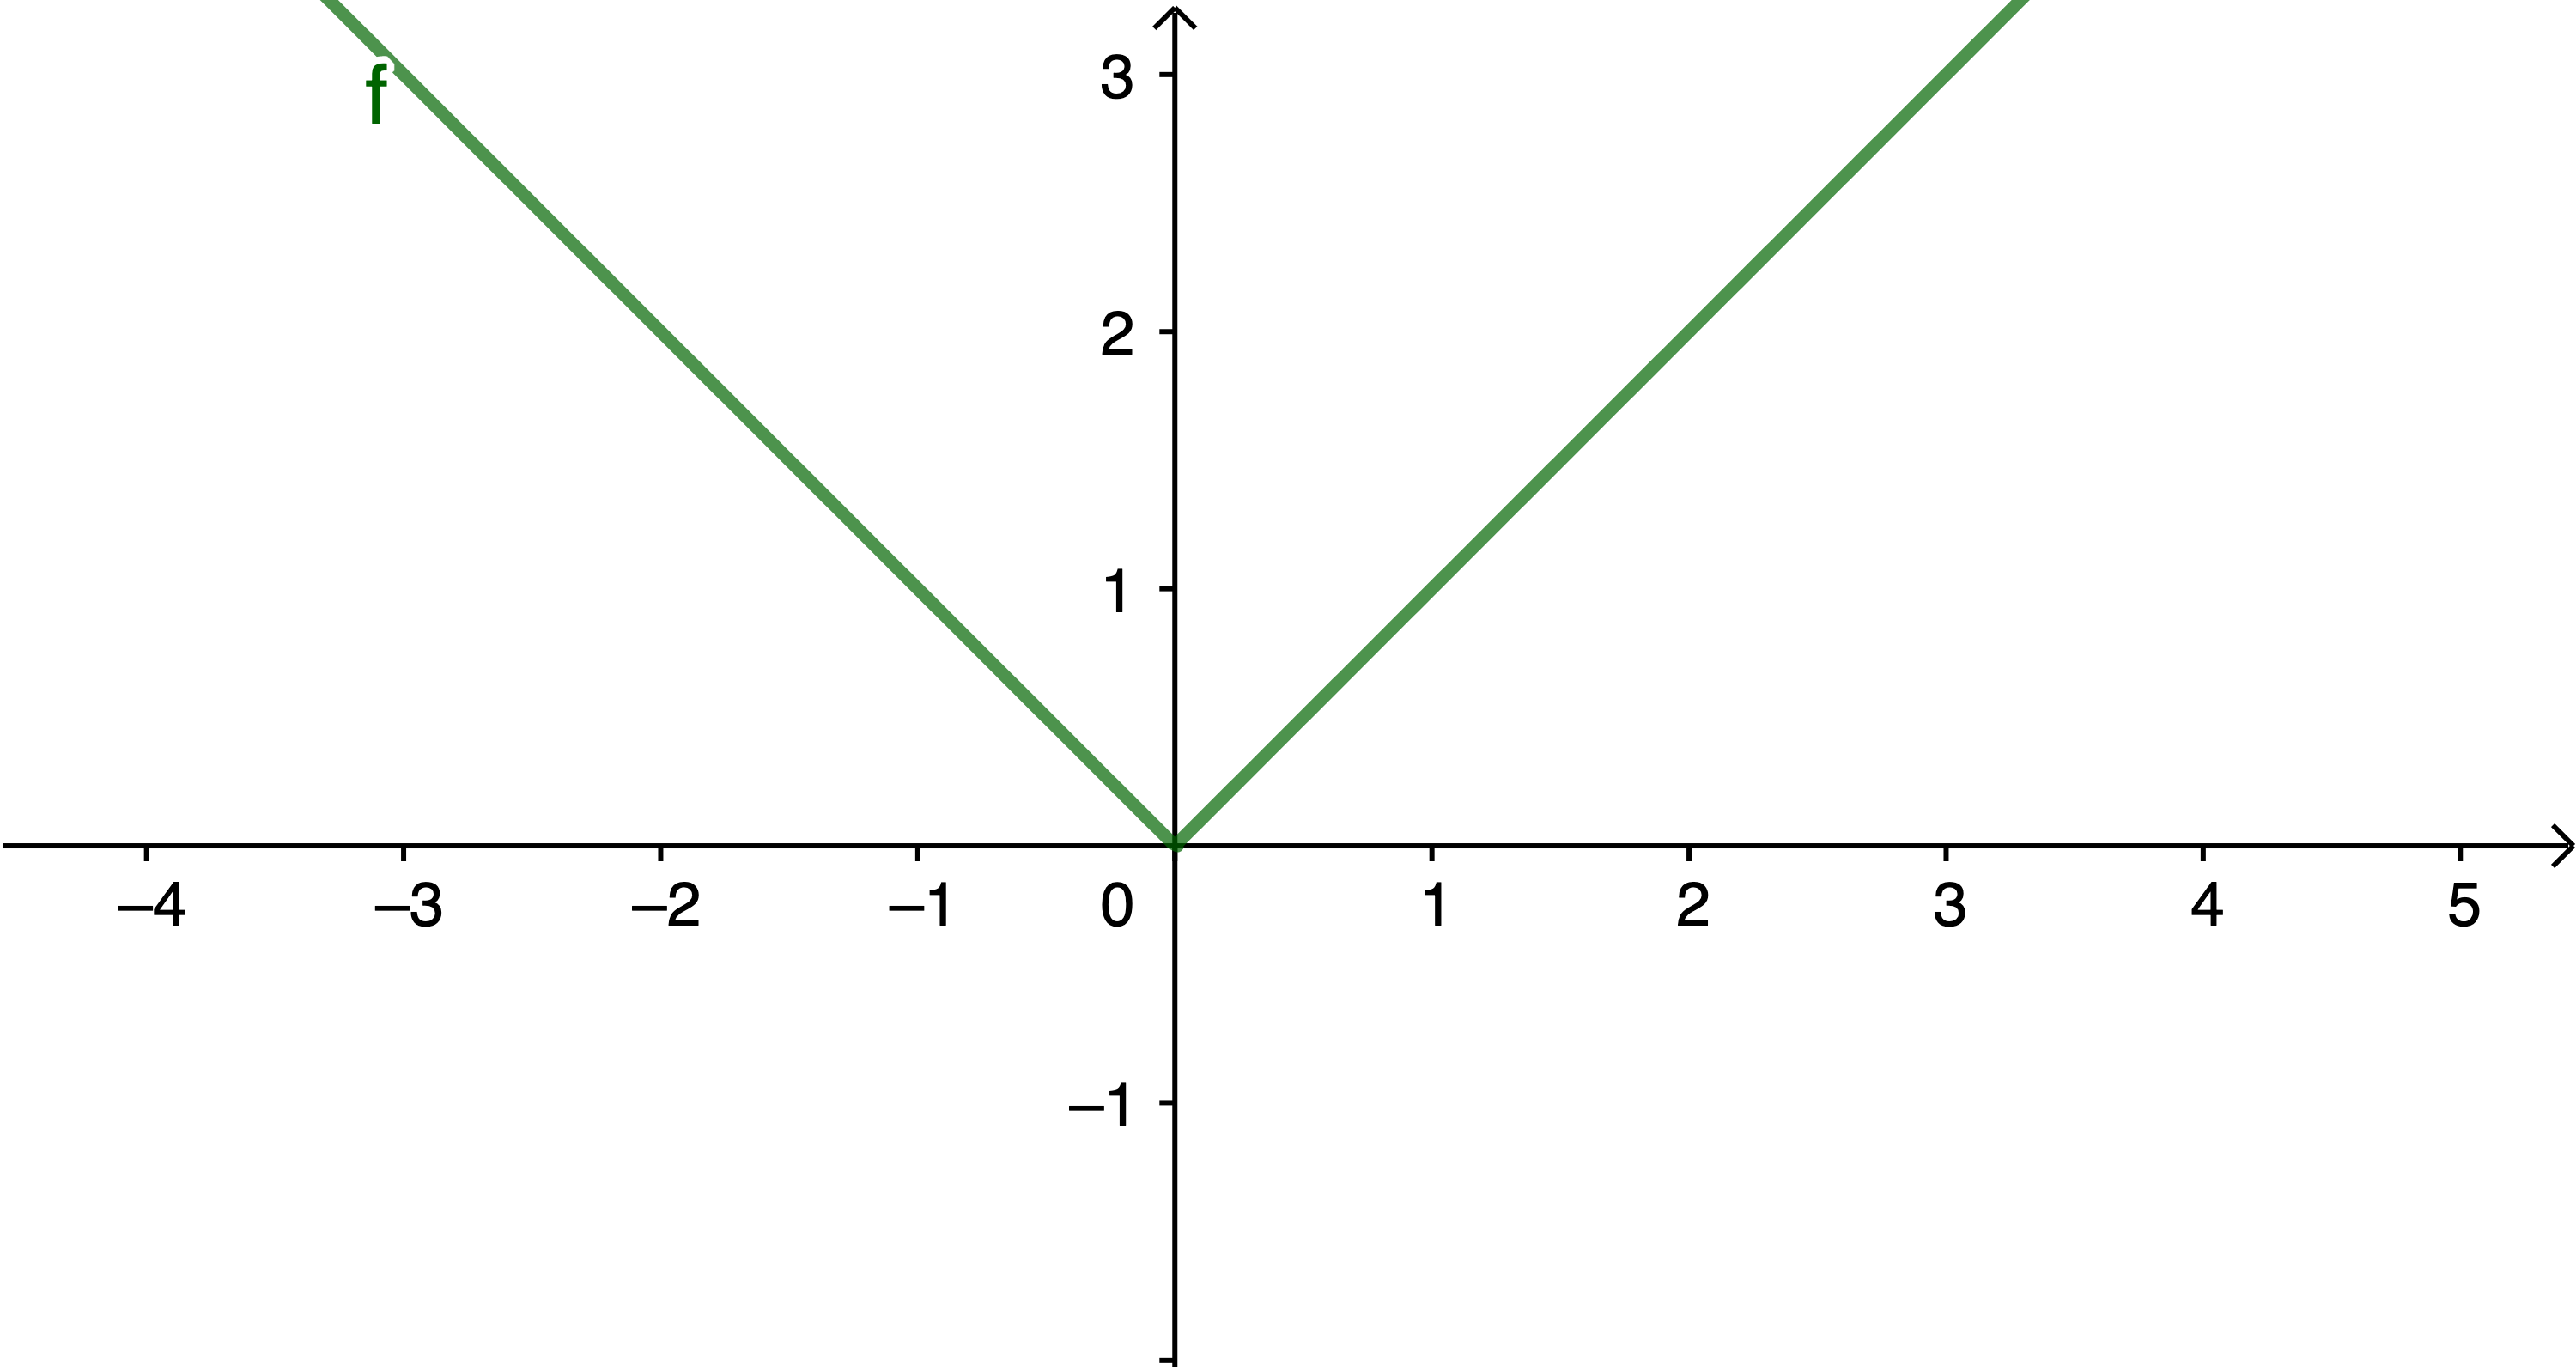
\includegraphics[scale=0.8]{media/abs.png}
    \end{center}
    \item 	Die Kehrwertfunktion  $p(x)=\frac{1}{x}$ ist trotz des Sprungs von $-\infty$ nach $+\infty$ stetig, weil die vermeintliche Sprungstelle $x=0$ ausserhalb des Definitionsbereichs $\mathbb{D}_p$ liegt.
    \begin{center}
        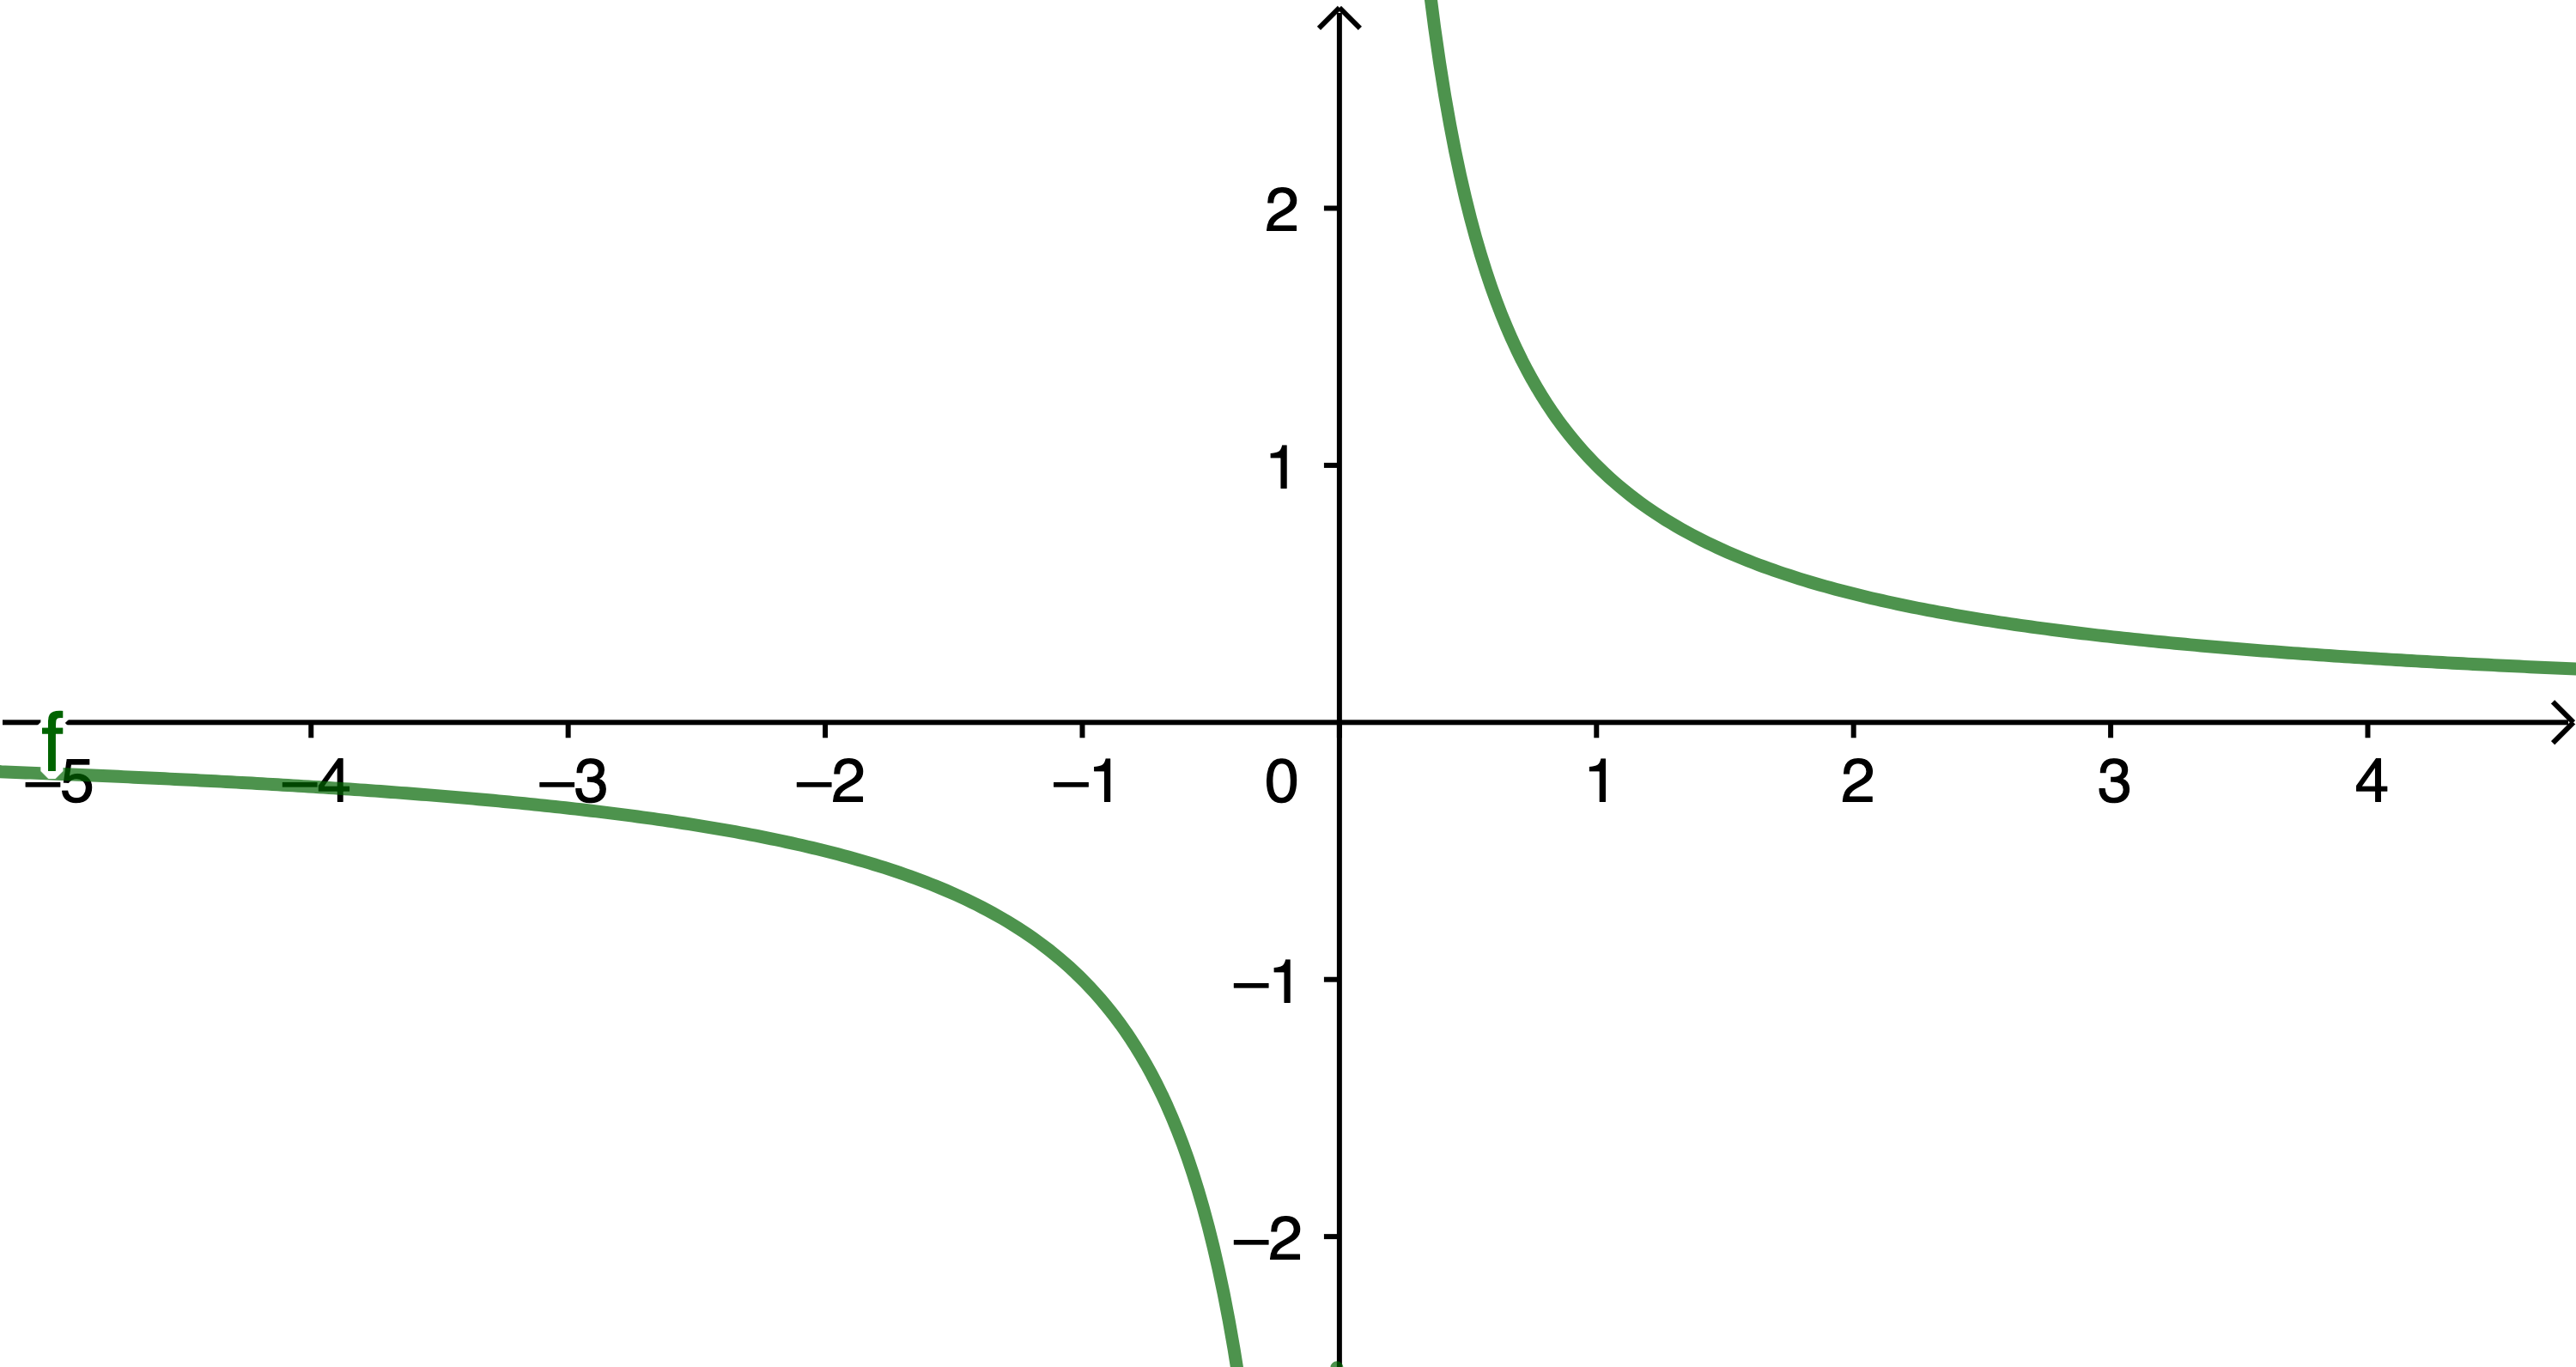
\includegraphics[scale=0.8]{media/kehrwert.png}
    \end{center}
    \end{enumerate}
     
\end{bsp}




\begin{ueb}{}{}
\begin{enumerate}
    \item Bestimme den links- und den rechtsseitigen Grenzwert der Funktion an der angegebenen Stelle. Ist die Funktion an dieser Stelle stetig?

    Bemerkung: Die Funktion $\lfloor x \rfloor$ ist die Abrundungsfunktion. Der Output ist die grösste ganze Zahl, die kleiner oder gleich $x$ ist.
    \begin{enumerate}
        \item $f(x)=x^2+x, \, a=3$
        \item  $f(x)=\lfloor x \rfloor, \, a=5$
        \item  $f(x)=\lfloor x-1 \rfloor, \, a=\frac{5}{2}$
        \item  $f(x)=\lvert x-5 \rvert, \, a=5$
        \item  $f(x)=\mathrm{sgn}(x-3), \, a=3$
        \item  $f(x)=\lfloor \cos(x)\rfloor, \, a=0$
    \end{enumerate}
    \item Gegeben ist die Funktion $f(x) = \left\{\begin{array}{ll}
        3-x, & x<2 \\\frac{x}{2}+1, &x\ge 2        
    \end{array}\right.$
    \begin{enumerate}
        \item Bestimme $\lim_{x\uparrow 4} f(x)$ und $\lim_{x\downarrow 4} f(x)$. Existiert $\lim_{x\to 4} f(x)$  ?
        \item Bestimme $\lim_{x\uparrow 2} f(x)$ und $\lim_{x\downarrow 2} f(x)$. Existiert $\lim_{x\to 2} f(x)$  ?
    \end{enumerate}
\end{enumerate}
\end{ueb}

\clearpage
\emph{Lösungen}
\begin{enumerate}
    \item Bestimme den links- und den rechtsseitigen Grenzwert der Funktion an der angegebenen Stelle. Ist die Funktion an dieser Stelle stetig?
    
    \begin{enumerate}
        \item $\lim\limits_{x \to 3^-} f(x) = 12$, \quad $\lim\limits_{x \to 3^+} f(x) = 12$ \newline $\Rightarrow$ Stetig
        \item $\lim\limits_{x \to 5^-} f(x) = 4$, \quad $\lim\limits_{x \to 5^+} f(x) = 5$ \newline $\Rightarrow$ Nicht stetig
        \item $\lim\limits_{x \to \frac{5}{2}^-} f(x) = 1$, \quad $\lim\limits_{x \to \frac{5}{2}^+} f(x) = 1$ \newline $\Rightarrow$  Stetig
        \item $\lim\limits_{x \to 5^-} f(x) = 0$, \quad $\lim\limits_{x \to 5^+} f(x) = 0$ \newline $\Rightarrow$ Stetig
        \item $\lim\limits_{x \to 3^-} f(x) = -1$, \quad $\lim\limits_{x \to 3^+} f(x) = 1$ \newline $\Rightarrow$ Nicht stetig
        \item $\lim\limits_{x \to 0^-} f(x) = 0$, \quad $\lim\limits_{x \to 0^+} f(x) = 0$ aber $\cos(0)=1$ \newline $\Rightarrow$ Nicht stetig
    \end{enumerate}
    
    \item Gegeben ist die Funktion 
    \[
        f(x) = \begin{cases} 
        3-x, & x<2 \\ 
        \frac{x}{2}+1, & x\geq 2 
        \end{cases}
    \]
    \begin{enumerate}
        \item $\lim\limits_{x \uparrow 4} f(x) = 3$, \quad $\lim\limits_{x \downarrow 4} f(x) = 3$ \newline $\Rightarrow$ Existiert mit Wert $3$
        \item $\lim\limits_{x \uparrow 2} f(x) = 1$, \quad $\lim\limits_{x \downarrow 2} f(x) = 2$ \newline $\Rightarrow$ Grenzwert existiert nicht
    \end{enumerate}
\end{enumerate}

\clearpage
Bei einer `asymptotischen Analyse' werden die Grenzwerte einer Funktion für $x\to\pm\infty$ und an allen Definitionslücken bestimmt. Damit kann man sich eine gute Vorstellung des Funktionsgraphen machen.

\begin{bsp}
    {Asymptotische Analyse der Funktion $f(x)= \frac{x^2-4}{x^2-5x+6}$}{}
    
    \vspace*{19cm}
\end{bsp}

\begin{ueb}
    {}{}
    Führe die asymptotische Analyse durch.
    \begin{enumerate}
        \item $f(x) = \frac{x^2-2x-3}{x^2-9}$
        \item $g(x) = \frac{x}{x^3-4x^2+4x}$
    \end{enumerate}

    Zeichne die entsprechenden Graphen mit Geogebra, um die Lösung zu überprüfen. 
\end{ueb}